

\section{Results}
\label{sec:results}

In order to conclude that our models actually learned, we needed to compare
our results to a baseline. We produced three measures with which to make
these comparisons: the coefficient of determination, mean absolute error, 
and mean squared error. \\

The coefficient of determination is also known as the $R^2$ score. This metric
returns a value between -1.0 and 1.0. A score of 0.0 denotes an equivalent
quality to that of a model which reports the expected value of the data set, 
regardless of the features, for every prediction \cite{scikit}. A negative score
is worse than a score of 0.0 and a positive score is better. The average scores
for white wine and red wine were 5.880 and 5.664 respectively. From this score
alone, we know that both of our models predicted the correct wine score
as determined by professional wine tasters better than a model
which only reports the average of a data set would. \\

With an $\alpha$ value of 0.0001, our randomized search cross-validation 
model which used ridge regression produced received an 
$R^2$ score of 0.2308. This validates that our model 
did indeed learn how to predict wine scores with some accuracy. A graphical
representation of the relationship between the $\alpha$ values and the $R^2$ score
for this method can be seen in Fig \ref{fig:R2ridge}. Additionally, our lasso model
performed better than the baseline $R^2$ score of 0.0 as well. The coefficient of
determination for lasso regression was 0.2139 for an $\alpha$ of $10^{-16}$, the smallest tested
$\alpha$. In general, smaller $\alpha$ values constructed more accurate models for
our lasso regression model. However these gains were at the loss of consideration
of certain features. The graph of $\alpha$ values for the lasso model versus the
coefficient of determination can be seen in Fig \ref{fig:LassoR2}.\\

\begin{figure}[htb]



  \centering  % centers the image in the column

  % replace the second argument below with your filename. I like to
  % place all my figures in a sub-directory to keep things organized
  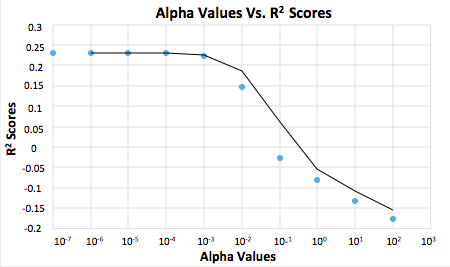
\includegraphics[width=0.47\textwidth]{figs/R2ridge.png}

  % *Every* figure should have a descriptive caption.
  \caption{The graph that represents $\alpha$ versus $R^2$ score. The same
  score was received for both white and red wine.}

  % The label is a handle you create so that you can refer to this
  % figure (using the \ref{} command) from other parts of your
  % document. LaTeX automatically renumbers figures and updates
  % references when you recompile, so you should do it this way rather
  % than hard-coding in references. Notice that I've also been
  % creating labels for the various sections in the document; I could
  % use \ref{} command to refer to those sections using their labels
  % too.
  \label{fig:R2ridge}

\end{figure}


\begin{figure}[htb]



  \centering  % centers the image in the column

  % replace the second argument below with your filename. I like to
  % place all my figures in a sub-directory to keep things organized
  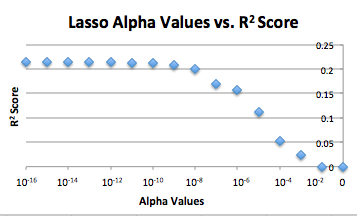
\includegraphics[width=0.47\textwidth]{figs/LassoR2.png}

  % *Every* figure should have a descriptive caption.
  \caption{The correlation between $\alpha$ and $R^2$ score for lasso regression.}

  % The label is a handle you create so that you can refer to this
  % figure (using the \ref{} command) from other parts of your
  % document. LaTeX automatically renumbers figures and updates
  % references when you recompile, so you should do it this way rather
  % than hard-coding in references. Notice that I've also been
  % creating labels for the various sections in the document; I could
  % use \ref{} command to refer to those sections using their labels
  % too.
  \label{fig:LassoAvS}

\end{figure}


For our primary model, the randomized search k-fold cross validation model,
we report the mean absolute error and the mean square error. A comparison
of these errors versus $\alpha$ values can be viewed in Fig \ref{fig:errorridge}.
These scores also tell us that our model is doing better than the baseline.
If all values in the data set were predicted to be the value of the average 
of the data, then the calculated mean and absolute squared errors would
be higher than those found in our ridge regression model. The calculated
errors can be viewed in Fig \ref{tab:baseline}. \\


\begin{figure}[htb]



  \centering  % centers the image in the column

  % replace the second argument below with your filename. I like to
  % place all my figures in a sub-directory to keep things organized
  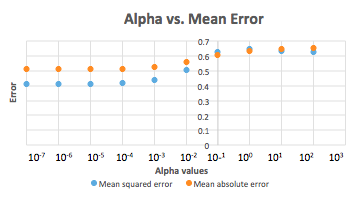
\includegraphics[width=0.47\textwidth]{figs/errorridge.png}

  % *Every* figure should have a descriptive caption.
  \caption{ $\alpha$ versus mean square and absolute errors for ridge regression.}

  % The label is a handle you create so that you can refer to this
  % figure (using the \ref{} command) from other parts of your
  % document. LaTeX automatically renumbers figures and updates
  % references when you recompile, so you should do it this way rather
  % than hard-coding in references. Notice that I've also been
  % creating labels for the various sections in the document; I could
  % use \ref{} command to refer to those sections using their labels
  % too.
  \label{fig:errorridge}

\end{figure}

\begin{figure}[htb]
  \centering % centers the entire table

  % The following line sets the parameters of the table: we'll have
  % three columns (one per 'c'), each
  % column will be centered (hence the 'c'; 'l' or 'r' will left or
  % right justify the column) and the columns
  % will have lines between them (that's the purpose of the |s between
  % the 'c's).
  \begin{tabular}{|c|c|c|} 
    \hline \hline % draws two horizontal lines at the top of the table
    $~$ & $Mean~Squared~Error$ & $Mean~Average~Error$\\ % separate column contents using the &
    \hline % line after the column headers
    $White$ & $0.6008$ & $0.5682$\\
    $Red$ & $0.6249$ & $0.6521$\\
    \hline \hline
  \end{tabular}

  % As with figures, *every* table should have a descriptive caption
  % and a label for ease of reference.
  \caption{Baseline error values for white and red wines.}
  \label{tab:baseline}
\end{figure}

At an $\alpha$ value of 0.001, our model produced a mean absolute error of 0.5135
and a mean squared error of 0.4148. These numbers are lower than those presented
in Fig \ref{tab:baseline}. We did not perform this set of experiments on the lasso regression,
as it was a later addition to our experiments.







